\setcounter{chapter}{5}

\chapter{定积分的应用}

定积分的应用往往针对的是所谓的{\kaishu 可加性}问题,在现实中这类问题很多,
例如:几何中的体积、面积,物理中的质量、转动惯量、外有引力等等。如果不使用
定积分的方法,通常需要根据不同函数自身的特点,采取一些针对性的方法(例如:求
面积时的割补法、力学中的等效原理等)。引入了定积分的概念和计算方法后,
很多此类的问题都可以以一种统一的模式来解决,从而为研究和解决实际问题提供
更为强大的数学工具,在数学和工程技术发展的历史上都是非常巨大的进步。

\section{微元法(元素法)}

{\bf 回顾:}定积分的构造思路

\begin{center}
	\resizebox{!}{5.5cm}{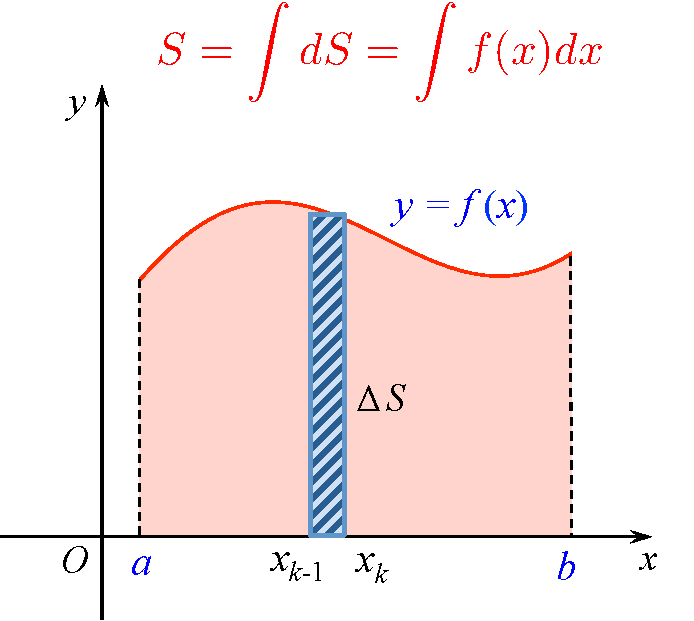
\includegraphics{./images/ch6/sumSSS.pdf}}

	{\kaishu 求曲边梯形的面积$S$}
\end{center}

\begin{enumerate}
  \setlength{\itemindent}{1cm}
  \item {\it 分割:}沿$x$轴方向分割积分区间,相应地将曲边梯形
  分割为与之对应的一系列不相重叠的小曲边梯形
  \item {\it 取近似:}用小矩形的面积$\Delta S$近似小曲边梯形面积
  \item {\it 做和:}求所有小矩形的面积总和$\sum \Delta S$,作为$S$的近似
  \item {\it 求极限:}使分法无限地趋于精细化,在一定条件下,$\lim\sum \Delta S=S$
\end{enumerate}

要使得上述过程的结果时有效的,需要以下的一些条件:首先,所求的和(在此为面积$S$)
是{\kaishu 可分的},也即$S$可以被分割为一系列与区间$[a,b]$的分法相对应的互不重叠的部分
(小曲边梯形的面积$\Delta S$),所有这些$\Delta S$的总和等于$S$,这个性质
也称为$S$关于区间$[a,b]$的{\kaishu 可加性};第二,对$\Delta $取近似时,
近似值与真实值的差应该是对应区间宽度$\Delta_k$的高阶无穷小,从而保证求和的极限
是$S$的精确值。

当然,我们知道,曲边梯形的面积是满足可加性的,而对于任何分段连续的函数,
由于其在$[x_{k-1},x_k]$上的函数值的最大变化量$|\Delta y_{\max}|$是随$\Delta x$趋于零
而趋于零的,故其面积近似的误差$|\Delta S_k-f(\xi_k)\Delta_k|\leq
|\Delta y_{\max}\Delta x|=\circ(\Delta x)$,故在我们的讨论中定积分的
可积性通常是不成问题的。

所谓定积分的{\bf 微元法},是对以上过程的另一种符号描述,是指与我们常用的微分和
积分运算符号更为一致,大致的过程如下:

\begin{enumerate}
  \setlength{\itemindent}{1cm}
  \item {\it 确定积分变量和长度微元(分割):}对任意的$x\in[a,b]$,取一个长度为$\d x$
  的区间;
  \item {\it 给出面积微元的表示(取近似):}$\d S=f(x)\d x$;
  \item {\it 利用积分计算总面积(做和求极限):}$S=\dint_D\d S=\dint_a^bf(x)\d x$。
\end{enumerate}

更抽象地可以与之类似的问题描述为:如果某个量$I$是与变量$x$的变化区间$[a,b]$
相对应也具有可加性的,并且其分割后的近似值$\Delta I$是关于$\Delta x$
的高阶无穷小,则可以采用如下的步骤计算它的值:

\begin{thx}
	{\bf 定积分的微元法(元素法)}
	\begin{enumerate}
		\item {\it 确定积分变量$x$和微元$\d x$:}任取$x\in[a,b]$和一个区间长度$\d x$;
  	    \item {\it 给出微元$\d I$的表示:}$\d I=f(x)\d x$;
  	    \item {\it 计算积分:}$I=\dint_a^bf(x)\d x$。
	\end{enumerate}
\end{thx}

\section{定积分的几何应用}

\subsection{平面区域面积}

{\bf 例:}计算两条抛物线$y^2=x$和$y=x^2$所围图形的面积。

{\bf 例:}计算两条抛物线$y^2=2x$与直线$y=x-4$所围图形的面积。

{\bf 例:}推导圆和扇形的面积公式。

\subsection{极坐标下的面积问题}

{\bf 例:}计算Archimedes螺线$\rho=a\theta\;(a>0)$
相应于$\theta$从$0$变到$2\pi$的一段弧与极轴所围的图形面积。

\begin{center}
	\resizebox{!}{4cm}{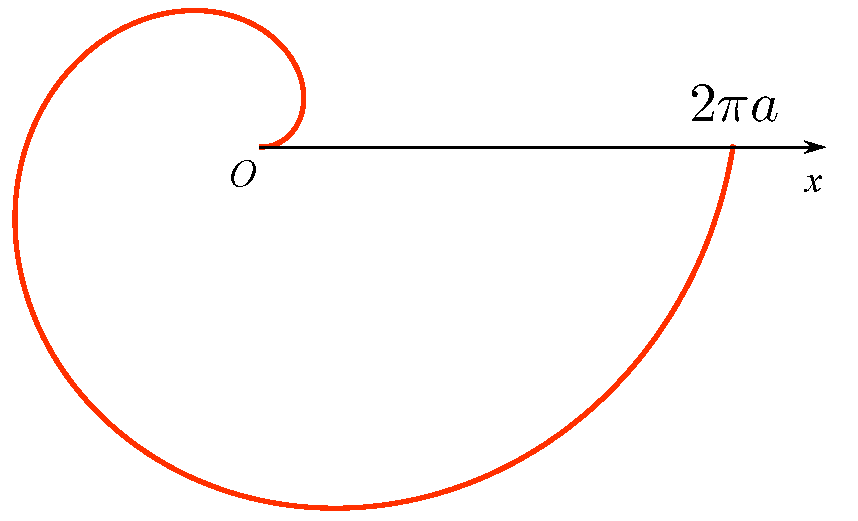
\includegraphics{./images/ch6/Achimedes.pdf}}
\end{center}

{\bf 例}(老羊三问题)
\begin{enumerate}[(1)]
  \setlength{\itemindent}{1cm}
  \item 半径为$a$的圆形水池,一只老羊被长为$ka(0<k\leq2)$的绳子拴在水池边缘,求
  老羊能吃到的草地面积
  \item 如果将水池围起来,老羊吃草时,绳子因为被绕在栅栏上而不能穿过水池,再求面积
  \item 在草场中央围一个半径为$a$的区域,要使内外的老羊吃到的草面积一样,$k$如何取
\end{enumerate}

[提示]:(1)
$$A=\pi k^2a^2-2\dint_{\arccos\frac k2}^{\pi}\df12(2a\cos\varphi)^2
\d\varphi$$
$$A=a^2\left[(k^2-1)\pi+(2-k^2)\arccos\df k2+\df k2
\sqrt{4-k^2}\right]$$
(2)
$$A=\df{\pi k^2a^2}2+2\dint_0^k\df12(ka-a\varphi)^2\d\varphi=k^2a^2
\left(\df{\pi}2+\df k3\right)$$
以上的$\varphi$为小园的圆心角
(3)$k=1.26$

\subsection{平面曲线的弧长}

{\bf 例:}求以下曲线的弧长
\begin{enumerate}[(1)]
  \setlength{\itemindent}{1cm}
  \item $y=\df 23x^{3/2}\;(a\leq x\leq b)$
  \item $x=a(t-\sin t),y=a(1-\cos t)\;(0\leq t\leq 2\pi)$
  \item $\rho=a\theta\;(a>0,\;0\leq t\leq 2\pi)$
\end{enumerate}

\subsection{旋转体的体积}

圆盘法:曲线$y=f(x)\;(x\in[a,b])$与$x=a,x=b,y=0$所围区域绕$x$轴旋转一周:
$$V=\dint_a^b\pi[f(x)]^2\d x$$

{\bf 例:}求椭圆$\df{x^a}{a^2}+\df{y^2}{b^2}=1$绕$x$轴旋转一周所得立体的体积。

圆柱壳法:$y=f(x)\;(x\in[a,b])$与$x=a,x=b,y=0$所围区域绕$y$轴旋转一周
$$V=2\pi\dint_a^bx|f(x)|\d x$$

{\bf 例:}计算由圆滚线$$x=a(t-\sin t),y=a(1-\cos t)\;(0\leq t\leq 2\pi)$$
和直线$y=0$所围图形分别绕$x$轴、$y$轴旋转一周所得立体的体积。

\subsection{旋转体的表面积}
曲线$y=f(x)\;(x\in[a,b])$绕$x$轴旋转一周:
$$A=2\pi \dint_a^by\d s=2\pi \dint_a^by\sqrt{1+(y')^2}\d x$$

[提示]:圆台的侧面积
$$A=\pi(r_1+r_2)l$$
其中$r_1,r_2$为上下底的半径,$l$为斜高(或母线长度)
$$\Delta A=2\pi(y+(y+\Delta y))\sqrt{(\Delta x)^2+(\Delta y)^2}
=2\pi y\sqrt{1+(y')^2}\Delta x+\circ(\Delta x)$$

\subsection{已知截面积的立体体积}

{\bf 例:}一平面经过半径为$R$的圆柱体的底面圆心,并与底面交角为$\alpha$
(如图所示),求该平面所截圆柱体

\begin{center}
	\resizebox{!}{4.5cm}{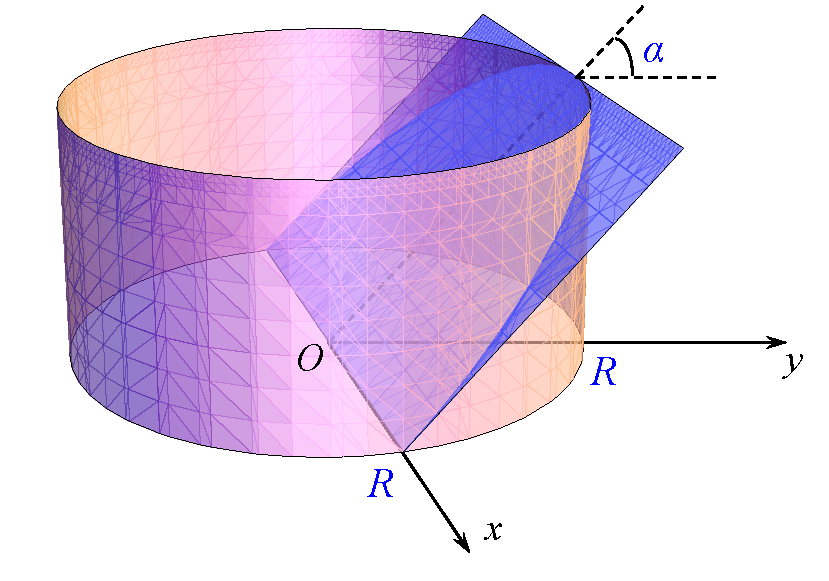
\includegraphics{./images/ch6/bucket.pdf}}
\end{center}

{\bf 例:}半径不等的两个木质球体,分别中间凿去一个以直径为轴的正圆柱体以及柱体下方的球冠,
剩下的环状部分高度均为$h$,问哪一个环状物体的体积更大。

[提示]:
$$V=\dint_{\sqrt{R^2-h^2}}^R2\pi x\sqrt{R^2-x^2}\d x=\df23\pi h^3$$
结果表明:剩余部分的体积与球半径无关!

{\bf 例:}试推导球的体积公式和球面上一块面积为$S$的球心锥的体积公式($rS/3$)

{\bf 例:}开口容器内的水在单位时间内的蒸发量与水的表面积成正比,证明:水的深度以常速率
下降且与容器形状无关。

[提示]:设水的表面积为$S$,则
$$\Delta V\approx S\Delta h\Rightarrow
\df{\Delta V}{\Delta t}\approx S\df{\Delta h}{\Delta t}$$
即
$$\df{\d V}{\d t}=S\df{\d h}{\d t}$$

\begin{ext}
	{\bf 课后作业}
	\begin{enumerate}
	  \item 设$S(t)$为直线$l_t:x+y=t(t\geq0)$下方位于正方形区域
	  $D:0\leq x\leq 1,0\leq y\leq 1$内的区域,求$\dint_0^xS(t)\d t$。
	  \item 计算下列曲线的弧长
	  \begin{enumerate}[(1)]
	    \item $y=\ln(1-x^2)$,$0\leq x\leq\df12$;
	    \item $\rho=a(1+\cos\theta)$,$0\leq\theta\leq2\pi$
	  \end{enumerate}
	  \item 设$D$是由曲线$y=\sin x+1$与三条直线$x=0,x=\pi,y=0$
	  所围成的曲边梯形,求$D$绕$x$轴旋转一周所围成的旋转体的体积。
	  \item 证明球冠(球缺)的体积公式:$V=\pi h\left(R-\df h3\right)$,其中$R$为球
	  的半径,$h<R$为球冠(球缺)的高。
	  \item 直线$y=x$将椭圆$x^2+3y^2=6y$分为两块,求两块的面积之比。
	  \item 求曲线$y=\sqrt x$的一条切线,使之与该曲线及$x=0$、$x=2$
	  共同所围面积最小。
	  \item 求圆滚线:$x=a(t-\sin t),y=a(1-\cos t)$的一拱($0\leq t\leq 2\pi$)
	  与横轴所围成的图形的面积,及其绕$x$轴旋转一周所得的旋转体的体积。
	  \item 求底面是半径为$R$的圆,而垂直于底面上一条固定直径的所有截面均为
	  等边三角形的立体的体积。
	\end{enumerate}
\end{ext}

\section{定积分的物理应用}

\subsection{平面物体的质心}
$y=f(x)(a<x<b)$密度均匀,其质心的横坐标为
$$\bar{x}=\df{\dint_a^bxf(x)\d x}{\dint_a^bf(x)\d x}$$

{\bf 例:}求右半圆的质心坐标。

{\bf 例:}$f(x)\in C[a,b]$且单调递增,证明:
$$\dint_a^bxf(x)\d x\geq\df{a+b}2\dint_a^bf(x)\d x$$

[提示]:物理意义:递增函数的形成的曲边梯形质心位于右侧。

[证1]:由$f(x)$单增,
$$\left(x-\df{a+b}2\right)\left[f(x)-f\left(
\df{a+b}2\right)\right]\geq0$$
两边积分即得。
\fin

注:$f\left(\df{a+b}2\right)\dint_a^b\left(x-\df{a+b}2\right)=0$

[证2]:记$c=\df{a+b}2$
\begin{align}
	\dint_a^b&(x-c)f(x)\d x\notag\\
	&=\left(\dint_a^c+\dint_c^b\right)(x-c)f(x)\d x\notag\\
	&=f(\xi_1)\dint_a^c(x-c)\d x+f(\xi_2)\dint_c^b(x-c)\d x\notag\\
	&=[f(\xi_1)-f(\xi_2)]\df{(b-a)^2}2\geq0\notag
\end{align}
\fin

\subsection{变力沿直线做功}

{\bf 例:}一圆柱形的水桶高$5m$,底半径$3$m,桶内装满水,问要将桶内的水全部抽出,
需要做多少功(设重力加速度$g=10N/kg$)。

{\bf 例:}在由电量为$+q$的电荷产生的电场中,沿某一轴向将一个单位正电荷由距离
$a$移动到距离$b$的位置,问在该过程中,电场力共对该电荷做了多少功?

{\bf 电场力:}
$$F=k\df{q_1q_2}{r^2}$$

\subsection{水压}

{\bf 例:}某个圆柱形油桶底半径为$R$,所装油密度为$\rho$,
现将其装满油后横放,求其端面承受的压力。

\subsection{万有引力}

{\bf 例:}设有一长度为$l$,线密度为$\mu$的均匀细直棒,在其中垂线上距离棒$a$
处有一质量为$m$的质点$M$,求该棒对质点$M$的引力。

[提示]:
\begin{align}
	F&=-\dint_{-\frac l2}^{\frac l2}\df{Gam\mu}{(a^2+y^2)^{\frac32}}\d y
	=-\dint_{-\arctan\frac l{2a}}^{\arctan\frac l{2a}}\df{Gam\mu}{(a^2+(a\tan
	t)^2)^{\frac32}}\d (a\tan t)\notag\\
	&=-\df{Gm\mu}a\dint_{-\arctan\frac l{2a}}^{\arctan\frac
	l{2a}}\cos t\d t=-\df{Gm\mu}a\left.\sin t\right|_{-\arctan\frac
	l{2a}}^{\arctan\frac l{2a}}\notag\\
	&=-\df{2Gm\mu}a\sin\left(\arctan\df l{2a}\right)\notag
\end{align}
注意到$\sin x=\df{\tan x}{\sec x}=\df{\tan x}{\sqrt{1+\tan^2 x}}$,故
$$\sin\left(\arctan\df l{2a}\right)=\df{\frac{l}{2a}}
{\sqrt{1+\left(\frac{l}{2a}\right)^2}}=\df{l}{\sqrt{4a^2+l^2}}$$
代回前式即得$F=-\df{2Gm\mu l}{a\sqrt{4a^2+l^2}}$。

\begin{ext}
	{\bf 课后作业}
	\begin{enumerate}
	  \item 长度为$l$的细杆,均匀带电,总电量为$q\,(q<0)$,若在杆的延长线上,
	  距离杆一端$x_0$处有一单位正电荷。现将单位正电荷从$x_0$处移动到无穷远,试求克服
	  电场力所作的功。
	  \item 星形线的参数方程为:$x=a\cos^3t,y=a\sin^3t$,设其上每一点处的密度
	  等于其到原点距离的$k$倍,在原点处放置一单位质点,求星形线在第一象限的部分对该
	  质点的引力。
	  \item 边长为$a$和$b$的矩形薄板,与水面成角度$\theta$斜沉于水中,长边
	  平行于水面,最低处深度为$h$,设$a<b$,水的密度$\rho=1$,求水对于薄板上侧
	  的总压力。
	  \item 一个物体按照$x=t^3$作直线运动,已知其所受阻力等于其速度平方的$1.5$倍,
	  求其从原点出发移动$1000$米时克服阻力所做的功。
	  \item 用铁锤将一铁钉击入木板,设木板对铁钉的阻力与铁钉已进入木板的深度成正比,
	  已知第一次敲击后,铁钉进入木板$1$cm,假设每次敲击所做的功相同,问第二次敲击
	  后,铁钉又将进入木板多少?
	  \item (选作)一个半径为$R$,圆心角为$\theta$的圆弧形细棒,其线密度为$\mu$,
	  在圆心处放置一单位质点,问细棒对该质点的引力大小为多少?方向如何?
	\end{enumerate}
\end{ext}

\newpage

\section*{作业参考解答}
% \addcontentsline{toc}{section}{作业参考解答}

\begin{center}
	\bf 6.2 定积分的几何应用
\end{center}

\bs

1. 设$S(t)$为直线$l_t:x+y=t(t\geq0)$下方位于正方形区域
$D:0\leq x\leq 1,0\leq y\leq 1$内的区域,求$\dint_0^xS(t)\d t$。

[解]:由$S(x)$的定义可得
$$S(t)=\left\{\begin{array}{ll}
	\df12t^2,& 0\leq t<1;\\ 1-\df12(2-t)^2, & 1\leq t <2;\\
	1,& t>2. 
\end{array}\right.$$
于是:当$0\leq x<1$时,
$$\dint_0^xS(t)\d t=\dint_0^x\df12t^2\d t=\df16x^3.$$
当$1<x\leq2$时,
$$\dint_0^xS(t)\d t=\dint_0^1\df12t^2\d t
+\dint_1^x\left[1-\df12(2-t)^2\right]\d t
=\df13+(x-1)+\df16(2-x)^3.$$
当$x>2$时,
$$\dint_0^xS(t)\d t=\dint_0^1\df12t^2\d t
+\dint_1^2\left[1-\df12(2-t)^2\right]\d t
+\dint_2^x1\d t
=x-\df13.$$
\fin

\bs

2.计算下列曲线的弧长

(1)$y=\ln(1-x^2)$,$0\leq x\leq\df12$

[解]:弧长微元
$$\d s=\sqrt{1+[y'(x)]^2}\d x=\df{1+x^2}{1-x^2}\d
x,\;(x\in\left[0,\df12\right]),$$
故所求弧长
$$s=\dint_0^{\frac12}\df{1+x^2}{1-x^2}\d x
=\dint_0^{\frac12}\left[\df1{1+x}+\df1{1-x}-1\right]\d x
=\left.\ln\df{1+x}{1-x}\right|_0^{\frac12}-\df12
=\ln3-\df12.$$

(2)$\rho=a(1+\cos\theta)$,$0\leq\theta\leq2\pi$

[解]:弧长微元
$$\d s=\sqrt{\rho^2(\theta)+[\rho'(\theta)]^2}\d\theta
=2a\left|\cos\df{\theta}2\right|\d\theta,\;\theta\in[0,2\pi],$$
故所求弧长
$$s=\dint_0^{2\pi}2a\left|\cos\df{\theta}2\right|\d\theta
=4a\dint_0^{\pi}\cos\df{\theta}2\d\theta
=8a.$$
\fin

\bs

3.设$D$是由曲线$y=\sin x+1$与三条直线$x=0,x=\pi,y=0$
所围成的曲边梯形,求$D$绕$x$轴旋转一周所围成的旋转体的体积。

[解]:如图
\begin{center}
	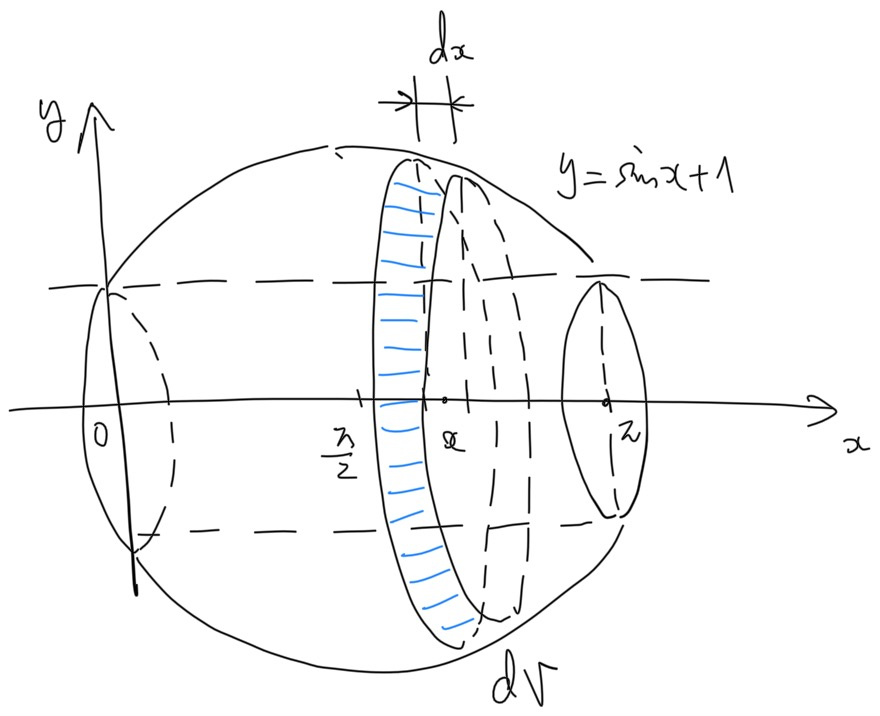
\includegraphics[width=7cm]{./images/ch6/sinx1cs.jpg}
	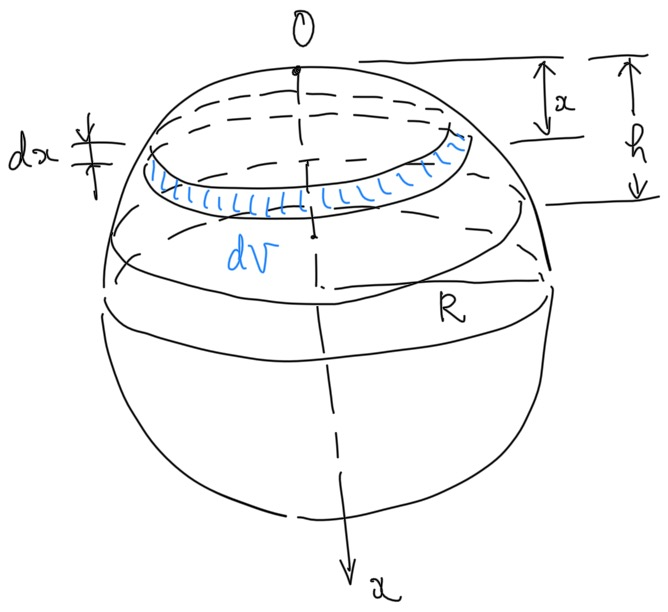
\includegraphics[width=6cm]{./images/ch6/topSp.jpg}
	
	{\kaishu 第3题图\hspace{6cm} 第4题图}
\end{center}
体积微元
$$\d V=\pi y^2\d x,$$
故所求体积
$$
	V=\dint_0^{\pi}\pi(\sin x+1)^2\d x=\df32\pi^2.
$$
\fin

\bs

4.证明球冠(球缺)的体积公式:$V=\pi h^2\left(R-\df{h}3\right)$,其中$R$为球
的半径,$h<R$为球冠(球缺)的高。

[证]:如图,体积微元
$$\d V=\pi[R^2-(R-x)^2]\d x=\pi(2Rx-x^2)\d x,$$
故球缺体积
$$V=\dint_0^h\pi(2Rx-x^2)\d x=\pi h^2\left(R-\df{h}3\right).$$
\fin

\bs

5.直线$y=x$将椭圆$x^2+3y^2=6y$分为两块,求两块的面积之比。

[解]:如图
\begin{center}
	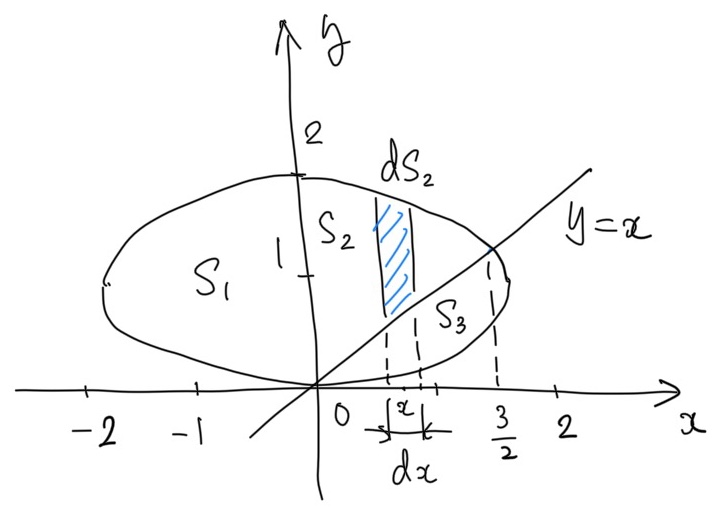
\includegraphics[width=7cm]{./images/ch6/ecXY.jpg}
	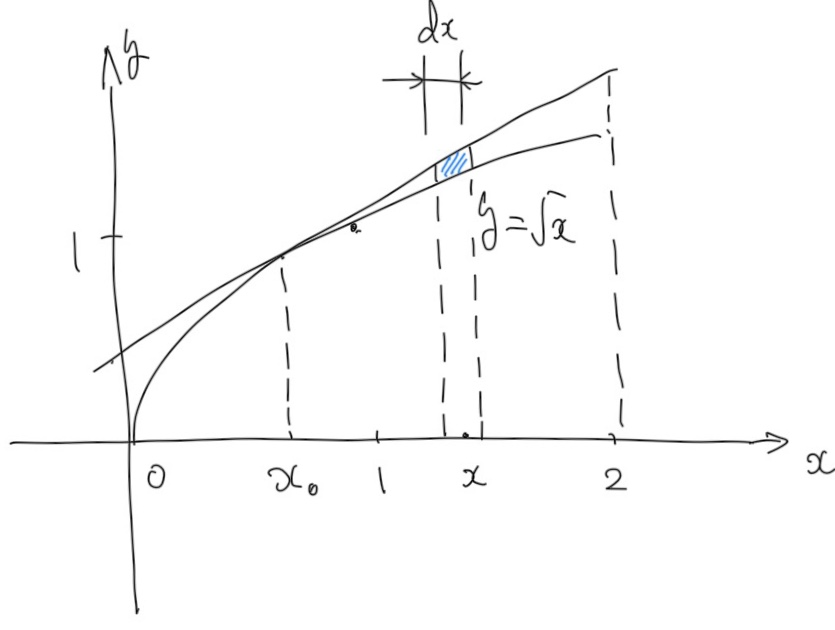
\includegraphics[width=7cm]{./images/ch6/ySqtXx.jpg}
	
	{\kaishu 第5题图\hspace{7cm} 第6题图}
\end{center}
体积微元
$$\d S_2=\left(1+\sqrt{1-\df{x^2}3}-x\right)\d x,\;x\in\left[0,\df32\right],$$
故
$$S_2=\dint_0^{\frac32}\left(1+\sqrt{1-\df{x^2}3}-x\right)\d x
=\df34+\df{\sqrt3}6\pi.$$
又$S_1=\sqrt3\pi$,故所求面积比为$\df{S_1-S_2}{S_1+S_2}=\df{10\sqrt3\pi-9}
{14\sqrt3\pi+9}$。
\fin

6.求曲线$y=\sqrt x$的一条切线,使之与该曲线及$x=0$、$x=2$
共同所围面积最小。

[解]:如图,任取曲线上一点$(x_0,\sqrt{x_0})$,过其的切线为
$$y=\sqrt{x_0}+\df1{\sqrt{2x_0}}(x-x_0),$$
进而体积微元
$$\d S=\left[\df1{\sqrt{2x_0}}(x-x_0)+\sqrt{x_0}-\sqrt{x}\right]\d
x,\;x\in[0,2],$$ 故所述体积
$$S=\dint_0^2\left[\df1{\sqrt{2x_0}}(x-x_0)+\sqrt{x_0}-\sqrt{x}\right]\d
x=\df{\sqrt2}{\sqrt{x_0}}+(2-\sqrt2)\sqrt{x_0}-\df{4\sqrt2}3.$$
对$S$求$x_0\in[0,2]$上的最小值可得,$x_0=2$时,该面积最小,为$\df{2\sqrt2}3-1$。
\fin

\bs

7.求圆滚线:$x=a(t-\sin t),y=a(1-\cos t)$的一拱($0\leq t\leq 2\pi$)
与横轴所围成的图形的面积,及其绕$x$轴旋转一周所得的旋转体的体积。

参见教材,解答略。

8.求底面是半径为$R$的圆,而垂直于底面上一条固定直径的所有截面均为
等边三角形的立体的体积。

[解]:如图
\begin{center}
	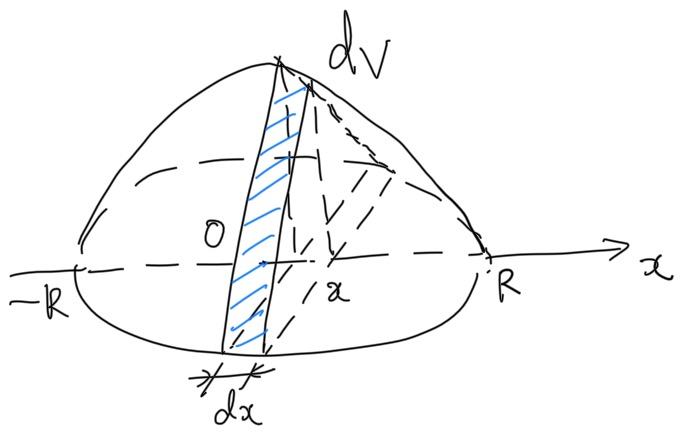
\includegraphics[width=7cm]{./images/ch6/rtSp.jpg}
\end{center}
体积微元
$$\d V=\sqrt3(R^2-x^2)\d x,\;x\in[-R,R],$$
故所求体积
$$V=\dint_{-R}^R\sqrt3(R^2-x^2)\d x=\df{4\sqrt3}3R^3.$$
\fin

\bs

1.长度为$l$的细杆,均匀带电,总电量为$q\,(q<0)$,若在杆的延长线上,
距离杆一端$x_0$处有一单位正电荷。现将单位正电荷从$x_0$处移动到无穷远,试求克服
电场力所作的功。

[解]:如图,
\begin{center}
	\resizebox{!}{2cm}{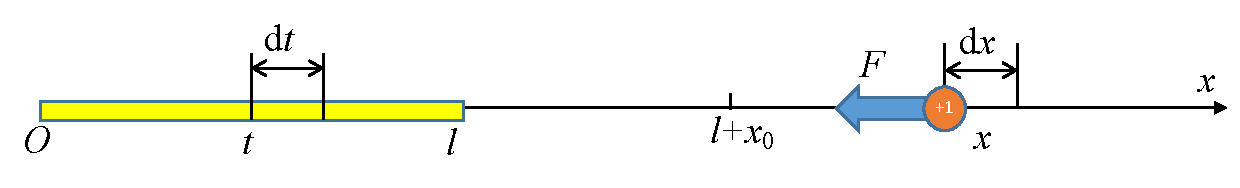
\includegraphics{./images/ch6/eMove.pdf}}
\end{center}
当单位正电荷位于$x(x>l)$处时,细杆上位置$t$处长度为$\d t$的一段对其产生的电场(吸引)力为
$$\d F=\df{kq\d t}{l(x-t)^2},\quad t\in[0,l]$$
故此时单位正电荷所受的总电场力为
$$F=\dint_0^l\df{kq\d t}{l(x-t)^2}=\df{kq}l\left(\df1{x-l}-\df1x\right).$$
克服该力的作用,单位正电荷向远处移动$\d x$,需要做的功为
$$\d W=F\d x=\df{kq}l\left(\df1{x-l}-\df1x\right)\d x,
\quad x\in[l+x_0,+\infty)$$
故所求克服电场力所需做的总功为
$$W=\dint_{l+x_0}^{+\infty}\df{kq}l\left(\df1{x-l}-\df1x\right)\d x
=\df{kq}l\ln\left(1+\df{l}{x_0}\right).$$
\fin

\bs

2.星形线的参数方程为:$x=a\cos^3t,y=a\sin^3t$,设其上每一点处的密度
等于其到原点距离的立方的$k$倍,在原点处放置一单位质点,求星形线在第一象限的部分对该
质点的引力。

[解]:如图,
\begin{center}
	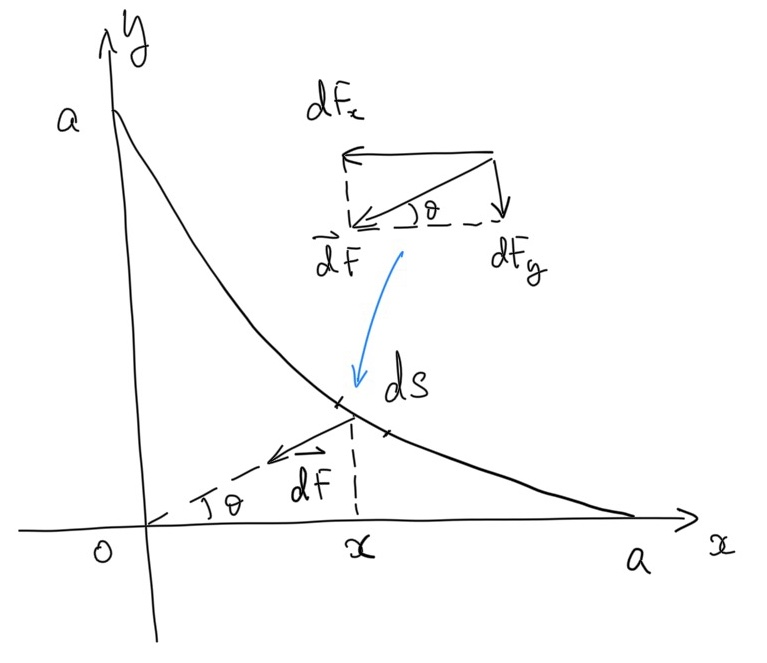
\includegraphics[width=8cm]{./images/ch6/starGr.jpg}
\end{center}
第一象限内的星形线对应于$t\in\left[0,\df{\pi}2\right]$,相应地,
弧长微元
$$\d s=\sqrt{(x'_t)^2+(y'_t)^2}\d t=3a\cos t\sin t\d t,$$
相应的质量微元
$$\d M=k(x^3+y^3)\d s,$$
其对原点处的单位质点的引力
$$|\bm{\d F}|=\df{G\d M}{x^2+y^2}=Gk\sqrt{x^2+y^2}\d s,$$
其分量
$$\d F_x=|\bm{\d F}|\cos\theta=Gkx\d s
=3a^2Gk\cos^4t\sin t\d t,$$
从而
$$F_x=\dint_0^{\frac{\pi}2}3a^2Gk\cos^4t\sin t\d t=\df{3a^2}5Gk.$$
注意到星形线关于$y=x$的对称性,易知必有
$$F_x=F_y=\df{3a^2}5Gk.$$
综上可知星形线对原点处的单位质点的引力大小为$\df{3a^2}{\sqrt2}Gk$,沿$y=x$的
方向指向原点。\fin

\bs

3.边长为$a$和$b$的矩形薄板,与水面成角度$\theta$斜沉于水中,长边
平行于水面,最低处深度为$h$,设$a<b$,水的密度$\rho=1$,求水对于薄板上侧
的总压力。

[解]:如图
\begin{center}
	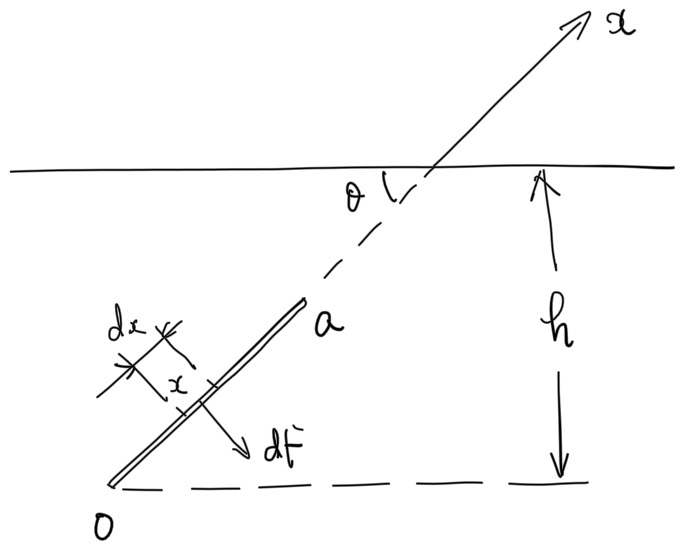
\includegraphics[width=7cm]{./images/ch6/waterPlane.jpg}
\end{center}
压力微元
$$\d F=g(h-x\sin\theta)b\d x,$$
故所求压力
$$F=\dint_0^ag(h-x\sin\theta)b\d x
=bg\left(ha-\df{a^2}2\sin\theta\right).$$
\fin

4.一个物体按照$x=t^3$作直线运动,已知其所受阻力等于其速度平方的$1.5$倍,
求其从原点出发移动$1000$米时克服阻力所做的功。

[解]:如图
\begin{center}
	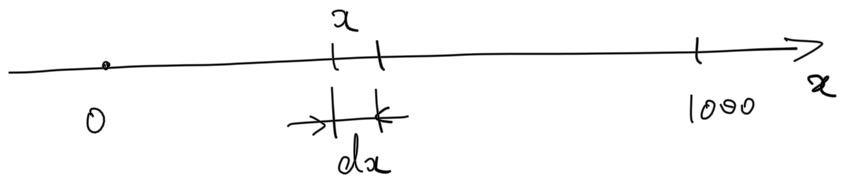
\includegraphics[width=9cm]{./images/ch6/moveSt.jpg}
\end{center}
功的微元
$$\d W=\df32(3t^2)^2\d x,$$
故所求总功
$$W=\dint_0^{10}\df32(3t^2)^2\d x=270000.$$
\fin

5.用铁锤将一铁钉击入木板,设木板对铁钉的阻力与铁钉已进入木板的深度成正比,
已知第一次敲击后,铁钉进入木板$1$cm,假设每次敲击所做的功相同,问第二次敲击
后,铁钉又将进入木板多少?

[解]:如图
\begin{center}
	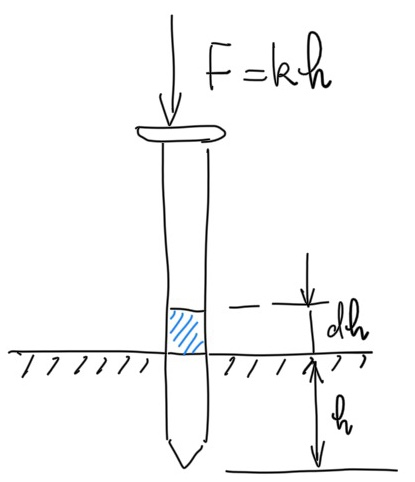
\includegraphics[width=6cm]{./images/ch6/nailSt.jpg}
\end{center}
功的微元
$$\d W=kh\d h,$$
由已知第一次敲击时所做的功
$$W_1=\dint_0^1kh\d h=\df k2,$$
根据假设每次敲击所做的功相同,设第二次敲击后到达的深度为$h_2$,则与之
相对应的功
$$W_2=\dint_1^{h_2}kh\d h=\df k2(h^2_2-1)=W_1=\df k2,$$
由此可解得$h_2=\sqrt2$。故第二次敲击后,铁钉又将进入目标的深度为
$\sqrt2-1$。\fin

\bs

6.一个半径为$R$,圆心角为$\theta$的圆弧形细棒,其线密度为$\mu$,
在圆心处放置一单位质点,问细棒对该质点的引力大小为多少?方向如何?

[解]:如图
\begin{center}
	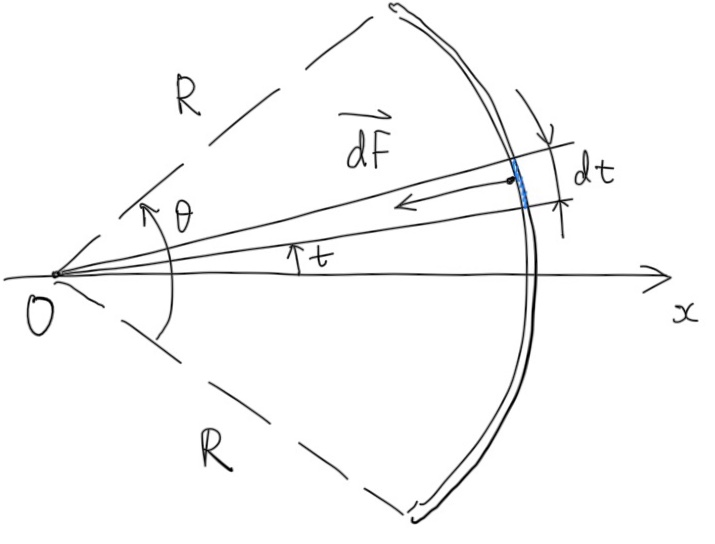
\includegraphics[width=6cm]{./images/ch6/theSphGr.jpg}
\end{center}
如图,引力微元
$$|\bm{\d F}|=\df{G\mu\d t}R,$$
其分量
\begin{align*}
	\d F_x&=|\bm{\d F}|\cos t=\df{G\mu\cos t\d t}R,\\
	\d F_y&=|\bm{\d F}|\cos t=\df{G\mu\sin t\d t}R,\\
\end{align*}
从而
\begin{align*}
	F_x&=\dint_{-\frac{\theta}2}^{\frac{\theta}2}\df{G\mu\cos t\d t}R
	=\df{2G\mu}{R}\sin\df{\theta}2,\\
	F_y&=\dint_{-\frac{\theta}2}^{\frac{\theta}2}\df{G\mu\sin t\d t}R=0,\\
\end{align*}
综上可知,所求引力大小为$\df{2G\mu}{R}\sin\df{\theta}2$,沿$x$轴指向原点方向。\fin